% ------------------------------------------------
%          FILE:  have-fun.tex
%       CREATED:  Dom seg 25 março de 2013 hs 9h
%   LAST CHANGE:  2013 Apr 06 03:48:23 PM
%        AUTHOR:  Sérgio Luiz Araújo Silva
%          SITE:  http://vivaotux.blogspot.com
%       TWITTER:  @voyeg3r
%         SKYPE:  sergioaraujosilva
% -------------------------------------------------

\chapter{Divirta-se ao aprender}

Colecione imagens engraçadas que contenham frases em inglês, piadas,
frases de efeito isso aumentará sua motivação para o estudo.

\begin{figure}[h!]
	\centering
	
\includegraphics[width=0.8\textwidth]{dna}
	\caption{dna}
\end{figure}

\vspace{0.3\baselineskip}
\noindent
{\footnotesize \ding{42} Hear a piece of information and three days later you will remember 10\% of it
 add a picture and you will remember 65\% -- Jonh Medina }

\section{Lista de video chats}
\label{sec:lista_de_video_chats}

Segue uma lista de sites em que podemos bater papo por vídeo, seja
cauteloso pois em alguns deles não há censura, sabendo disso faça suas
escolhas e boa diversão:

\begin{verbatim}
	http://www.tinychat.com/
	http://omegle.com/
	http://www.6rounds.com/
	http://www.tokbox.com
	http://www.anybodyoutthere.com/
	http://www.ekko.tv/
	http://www.palbee.com/
	http://vawkr.com/
	http://www.mebeam.com/
	http://chatroulette.com/
\end{verbatim}

\vspace{0.3\baselineskip}
\noindent
{\footnotesize \ding{42} ``The future belongs to those who believe in the beauty of their dreams''.  Eleanor Roosevelt  }


% section lista_de_video_chats (end)

\section{Ted Talks}
\label{sec:ted_talks}

Que tal aprender inglês assistindo excepcionais palestras com ou sem
legendas o nome do site é Ted Talks e o endereço é este:  \href{http://www.ted.com}{http://www.ted.com}

\begin{figure}[h!]
	\centering
	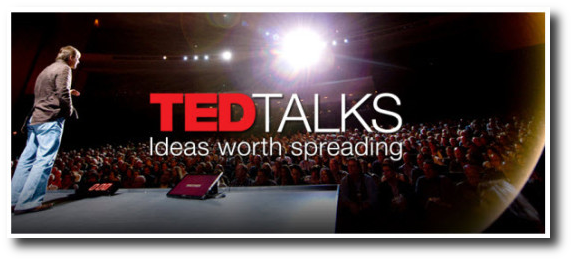
\includegraphics[width=0.8\textwidth]{ted-talks}
	\caption{ted-talks}
\end{figure}

TED (acrônimo para Technology, Entertainment, Design; Tecnologia,
Entretenimento, Design em português) é uma fundação privada sem fins
lucrativos dos Estados Unidos mais conhecida por suas conferências na
Europa, Ásia e Estados Unidos destinadas à disseminação de ideias.
Segundo as palavras da própria organização, “ideias que valem serem
disseminadas”.  As apresentações de Ted Talks são limitadas a dezoito
minutos, e os vídeos são amplamente divulgados na Internet.

O grupo foi fundado em 1984, e a primeira conferência Ted talks
aconteceu em 1990. Originalmente influenciada pelo Vale do Silício,
sua ênfase era tecnologia e design, mas com o aumento da popularidade
os temas abordados passaram a ser mais amplos, abrangendo quase todos
os aspectos de ciência e cultura. Entre os palestrantes no Ted talks
estão Bill Clinton, Al Gore, Gordon Brown, Richard Dawkins, Bill
Gates, os fundadores da Google, Billy Graham e diversos ganhadores do
Prêmio Nobel. Referência:
\href{http://www.hirondino.com/ted-talks/}{http://www.hirondino.com/ted-talks/}

O site disponibiliza links para baixar cada palestra permitindo ainda
selecionar como será a legenda e a qualidade do material baixado. uma
palestra recomendada fala sobre a febre do Inglês ao redor do mundo:
\href{http://goo.gl/bdwUJ}{http://goo.gl/bdwUJ}

% section ted_talks (end)
